\documentclass[class=article, crop=false, draft=true]{standalone}
\usepackage{graphicx}
\graphicspath{{../Figures}}

\usepackage{amsmath}

\usepackage{cleveref}

\begin{document}
As stated in the introduction, this report and the project it is written about are heavily based on \cite{specialization}. This was intended from the start. The goal of the specialization project was to provide a baseline to work from for this thesis.

Because of their highly interconnected nature, the specialization project is summarized here in some detail to provide appropriate background. As mentioned in the previous chapter, the specialization project is also included in appendix \ref{app:spec}

%equations, bib. \\
\section{Plan Sea}
The Plan Sea Project is a student-driven project with the goal of creating a solution to remove plastic from the seafloor. It is described in detail in the specialization project. In short, the current solution for the Plan Sea project can be broadly divided into three parts: A surface vessel that acts as an operations platform, an underwater gripper that is able to detect and grip plastic on the seafloor, and a basket to collect the plastics for the gripper. A sketch of the Plan Sea project can be seen in \cref{fig:overview}. The collection basket has been postponed to focus on the primary parts of the project.

\begin{figure}
    \centering
    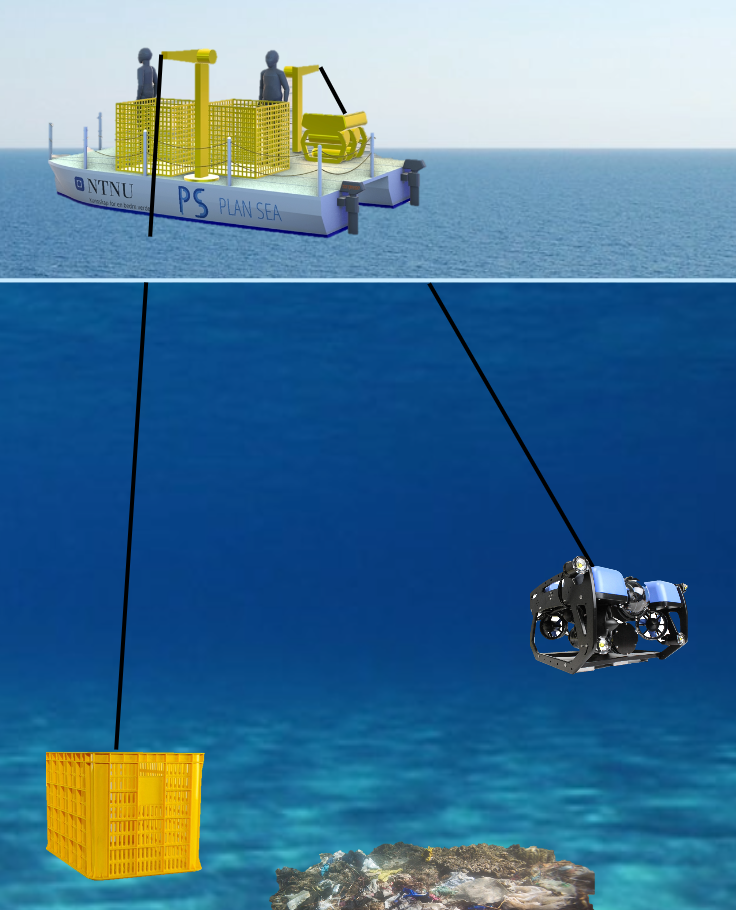
\includegraphics{overview}
    \caption{A rough overview sketch of the Plan Sea project proposed solution, credit \cite{specialization}}
    \label{fig:overview}
\end{figure}

The Plan Sea project is described in greater detail in \cite{specialization} and will thus not be further described here.

\section{Specialization Project}
The specialization project (\cite{specialization}) focused on making the framework for this thesis and for further work on the Plan Sea project in general.

Originally, the goals of the specialization project were as follows:
\begin{enumerate}
\item Create a simulation to be used in later work
\item Validate the performance of the simulation
\item Create a rudimentary control system for the simulation that can be further developed later
\item Do basic research that can be implemented in this thesis
\end{enumerate}
These goals were achieved with great success. Here is a short summary of each goal and its results.

\subsection{Creating the simulation}
\label{sec:basic_sim}
It was clear from the problem statement of the specialization project that a simulation was necessary. A control system without anything to control is not much use to anyone. The simulation would provide a plant for the control system, allowing at least basic development and testing of a seagoing vessel while staying warm and dry on land. With it clear that a simulation is necessary, a question arises: is it better to build a simulation from scratch or to use an existing framework?

When creating a framework from scratch, the developer has full control of everything. This is excellent for experienced developers in well-supported teams. A from-scratch solution could simulate exactly what is needed and in the exact level of detail needed. However, creating a simulation from scratch requires a lot of in-depth knowledge about many topics, including computation, physics, hydrodynamics, program optimization and more. In reality, this is a multi-person job simply due to the knowledge requirements.

Using an existing framework has the benefit of being practically a ready to use solution. It also avoids the issues of the from-scratch solution because these frameworks are generally made by large groups of people with all the in-depth knowledge necessary. The main drawbacks of using ready-made solutions are licensing costs and the learning curve of the simulation framework and its workings.

From the above, it was concluded that a commercial solution would be preferable, especially considering the fact that the simulation in question would require good handling of hydrodynamics and wire simulations, two notoriously difficult simulation topics. Additionally, using a finished commercial simulation solution would make it so the specialization project could focus on implementation. If it was decided that a from-scratch solution was to be made, the specialization project would likely primarily be about the programming of the simulator rather than the development of the control system. Preferably the simulation framework would be usable through code, not only through proprietary software. This requirement would make it easier to interface towards the simulation with the control system once that is implemented. Also, the simulation code should preferably be scriptable with Python due to the candidate's preference for the langauge.

Given all the above, the simulation framework AGX Dynamics made by Algoryx AB was chosen. The framework has modules for wire simulation, including winching movements. It also has a hydrodynamics package for handling buoyancy of the vessels. Additionally, AGX Dynamics is made to interface with ROS2 which would become a bonus for this project. This is elaborated upon in \cref{sec:simulation_work}

The Plan Sea project is based on two vessels. These were implemented into the simulation separately. The surface vessel(USV) was implemented as a simplified version of the designed hull.  The ROV was implemented as a simple box with  the appropriate dimensions. The basic setup can be seen in  \cref{fig:display}. Due to the demands of the Plan Sea project, the ROV would be negatively buoyant and hanging by a tether from the surface vessel. This was done to increase the lifting capacity of the ROV and is further discussed in \citet{specialization}.

\begin{figure}
    \centering
    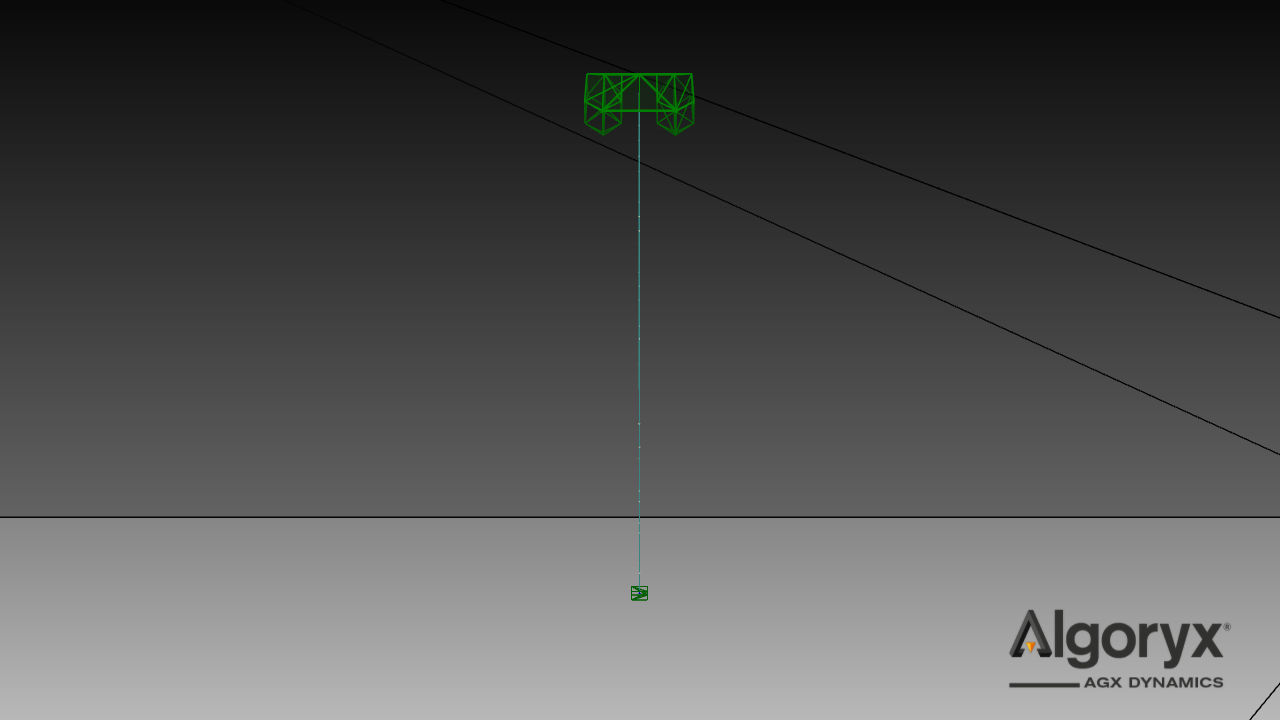
\includegraphics{sim-display}
    \caption{The display output from the simulation software with the two vessels implemented. Credit \cite{specialization}}
    \label{fig:display}
\end{figure}

\subsection{Validating the simulation}
The simulation was validated by comparing the tension measured in the tether to a calculated drag force that would be expected. The surface vessel would be moving at constant speed and the ROV dragged behind. This was done at several speeds, and the tension was measured both on average and as a function of time. The measured tension was then compared with a manually calculated drag force using the drag equation. The simulation was found to perform within \(\pm 20\%\) of the calculated drag, which given the assumptions made was concluded to be well within reasonable limits. Further discussion of this can be seen in section 4.2 of \citet{specialization}

\subsection{Creating a control system}
% A control system is a simplified abstraction of all the logic that is behind actually controlling a system. A "system" in this sense is any collection of real-world, digital, chemical or mechanical parts that accept some sort of affecting input and provide some resultant output. In this case, the movement of the vessels are the system of interest. The inputs of the system is the commands given to thrusters, cranes, or other means of moving the vessel, while the output of the system is the physical movement of the vessels and their components in space.

In the specialization project, the control system was implemented directly in the same script as the simulation ran on. This was not ideal, but it did work for a proof of concept. As it was implemented, it could control both the heading of the USV towards its waypoint as well as its total force applied. It was implemented as navigating to a list of points, changing to the next point after it reached some steady state around the current one. The movement of the ROV and crane was not controlled in the control system achieved in the specialization project.

Originally, implementing the control system using ROS2 was a goal of the specialization project. this was removed near the middle of the project due to the complexity of setting up the required framework. ROS2 stands for Robot Operating System 2 and is not really an operating system. ROS2 is a framework for communication between separate nodes of a larger control system. It allows for systems to be easily expanded or moved between different settings and developers. Especially helpful for the Plan Sea project would be the ability to make the simulation and the real-world vessel interchangable. By ensuring that the two communicated through the same channels with the same format of data, the control system outside of the plant would be able to control either of the two. This would allow for the same identical control system, tuned and tested in simulation, to be used almost immediately in the real world.

Due to time constraints and difficulty in setting up a working work-environment for ROS2, it was omitted from the specialization project and remained for the project in this thesis. The implementation of ROS2 is further discussed in \cref{sec:simulation_work}

\section{New Problem Statement}
\label{sec:problem_statement}
With the baseline of the specialization project, this project can come with its own problem statement that it attempts to solve for.

\begin{itemize}
\item Decouple the control system from the simulation and implement it in ROS2
\item Expand the control system to include winch and ROV movement
\item Create a human-machine interface/graphical user interface for the control system
\item Test that the new control system and simulation work well enough for further development
\end{itemize}

\end{document}
